\documentclass{standalone}
\usepackage{tikz}
\usetikzlibrary{patterns, positioning}

\begin{document}
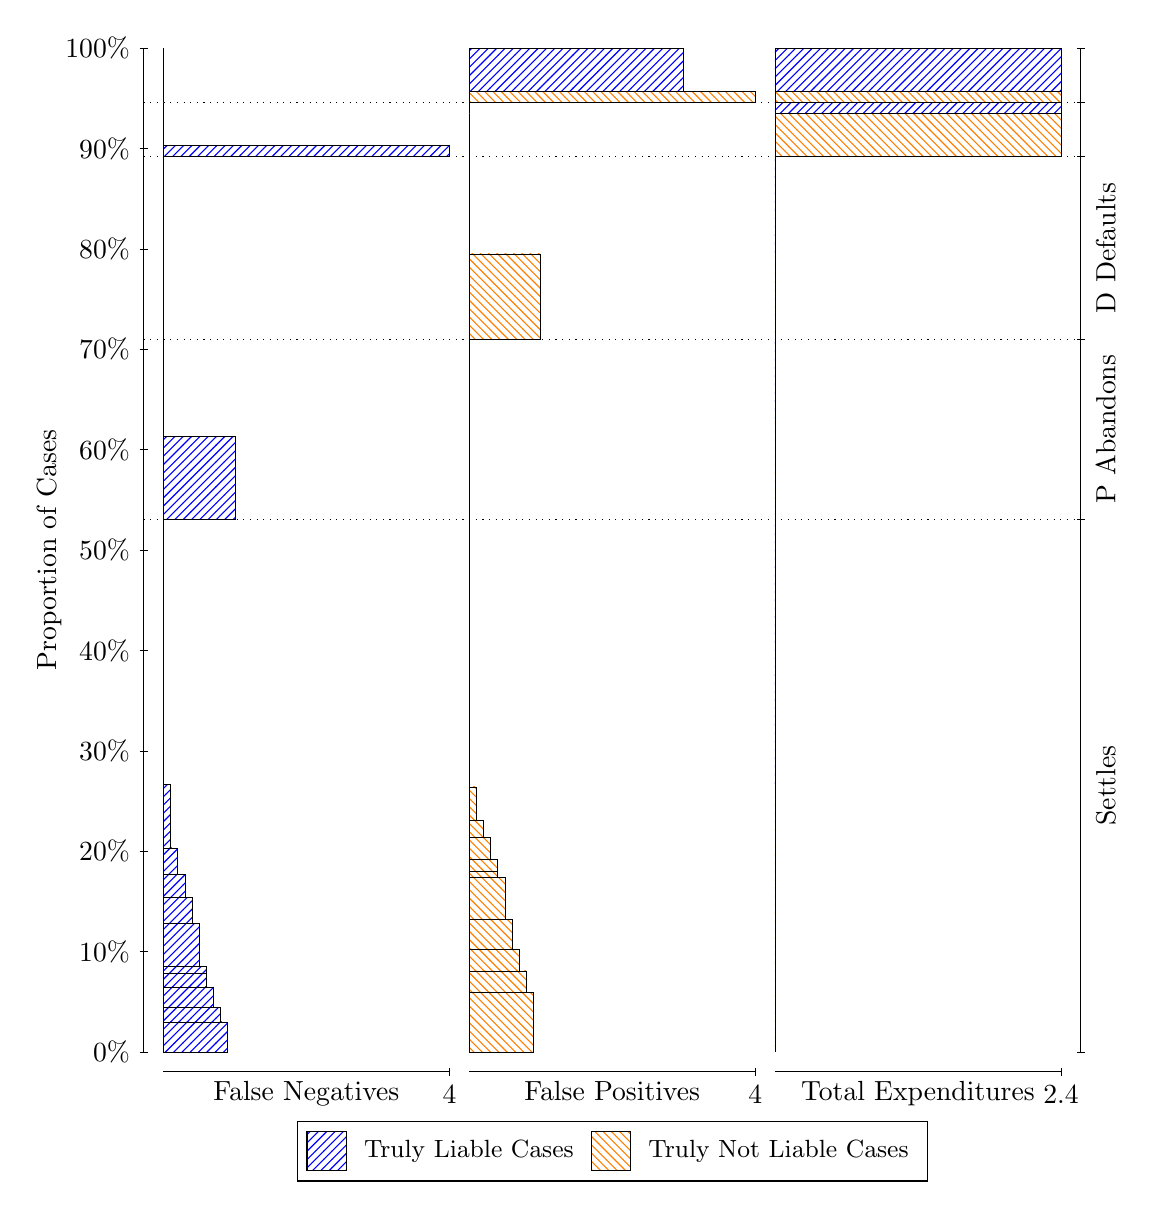
\begin{tikzpicture}
\draw[black, very thin] (1.5,1.75) -- (1.5,14.5);
\node[rotate=90, anchor=center] at (0.3, 8.125) {Proportion of Cases};
\draw[black, very thin] (1.45,1.75) -- (1.55,1.75);
\node[anchor=east] at (1.45, 1.75) {0\%};
\draw[black, very thin] (1.45,3.025) -- (1.55,3.025);
\node[anchor=east] at (1.45, 3.025) {10\%};
\draw[black, very thin] (1.45,4.3) -- (1.55,4.3);
\node[anchor=east] at (1.45, 4.3) {20\%};
\draw[black, very thin] (1.45,5.575) -- (1.55,5.575);
\node[anchor=east] at (1.45, 5.575) {30\%};
\draw[black, very thin] (1.45,6.85) -- (1.55,6.85);
\node[anchor=east] at (1.45, 6.85) {40\%};
\draw[black, very thin] (1.45,8.125) -- (1.55,8.125);
\node[anchor=east] at (1.45, 8.125) {50\%};
\draw[black, very thin] (1.45,9.4) -- (1.55,9.4);
\node[anchor=east] at (1.45, 9.4) {60\%};
\draw[black, very thin] (1.45,10.675) -- (1.55,10.675);
\node[anchor=east] at (1.45, 10.675) {70\%};
\draw[black, very thin] (1.45,11.95) -- (1.55,11.95);
\node[anchor=east] at (1.45, 11.95) {80\%};
\draw[black, very thin] (1.45,13.225) -- (1.55,13.225);
\node[anchor=east] at (1.45, 13.225) {90\%};
\draw[black, very thin] (1.45,14.5) -- (1.55,14.5);
\node[anchor=east] at (1.45, 14.5) {100\%};

\draw[black, very thin] (13.4,1.75) -- (13.4,14.5);
\draw[black, very thin] (13.35,1.75) -- (13.45,1.75);
\node[anchor=west] at (13.35, 1.75) {};
\draw[black, very thin] (13.35,8.5164) -- (13.45,8.5164);
\node[anchor=west] at (13.35, 8.5164) {};
\draw[black, very thin] (13.35,10.802) -- (13.45,10.802);
\node[anchor=west] at (13.35, 10.802) {};
\draw[black, very thin] (13.35,13.121) -- (13.45,13.121);
\node[anchor=west] at (13.35, 13.121) {};
\draw[black, very thin] (13.35,13.811) -- (13.45,13.811);
\node[anchor=west] at (13.35, 13.811) {};
\draw[black, very thin] (13.35,14.5) -- (13.45,14.5);
\node[anchor=west] at (13.35, 14.5) {};

\draw[black, very thin, pattern color=blue, pattern=north east lines] (1.75,1.75) rectangle (2.5675,2.1326);
\draw[black, very thin, pattern color=blue, pattern=north east lines] (1.75,2.1326) rectangle (2.4767,2.3201);
\draw[black, very thin, pattern color=blue, pattern=north east lines] (1.75,2.3201) rectangle (2.3858,2.5753);
\draw[black, very thin, pattern color=blue, pattern=north east lines] (1.75,2.5753) rectangle (2.295,2.7519);
\draw[black, very thin, pattern color=blue, pattern=north east lines] (1.75,2.7519) rectangle (2.295,2.835);
\draw[black, very thin, pattern color=blue, pattern=north east lines] (1.75,2.835) rectangle (2.2042,3.3782);
\draw[black, very thin, pattern color=blue, pattern=north east lines] (1.75,3.3782) rectangle (2.1133,3.7099);
\draw[black, very thin, pattern color=blue, pattern=north east lines] (1.75,3.7099) rectangle (2.0225,4.0083);
\draw[black, very thin, pattern color=blue, pattern=north east lines] (1.75,4.0083) rectangle (1.9317,4.3421);
\draw[black, very thin, pattern color=blue, pattern=north east lines] (1.75,4.3421) rectangle (1.8408,5.15);
\draw[black, very thin, pattern color=orange, pattern=north west lines] (1.75,5.15) rectangle (1.75,8.5164);
\draw[black, very thin, pattern color=blue, pattern=north east lines] (1.75,8.5164) rectangle (2.6583,9.5675);
\draw[black, very thin, pattern color=orange, pattern=north west lines] (1.75,9.5675) rectangle (1.75,10.802);
\draw[black, very thin, pattern color=orange, pattern=north west lines] (1.75,10.802) rectangle (1.75,11.886);
\draw[black, very thin, pattern color=blue, pattern=north east lines] (1.75,11.886) rectangle (1.75,13.121);
\draw[black, very thin, pattern color=blue, pattern=north east lines] (1.75,13.121) rectangle (5.3833,13.264);
\draw[black, very thin, pattern color=orange, pattern=north west lines] (1.75,13.264) rectangle (1.75,13.811);
\draw[black, very thin, pattern color=orange, pattern=north west lines] (1.75,13.811) rectangle (1.75,13.954);
\draw[black, very thin, pattern color=blue, pattern=north east lines] (1.75,13.954) rectangle (1.75,14.5);
\draw[black, very thin, pattern color=orange, pattern=north west lines] (5.6333,1.75) rectangle (6.4508,2.504);
\draw[black, very thin, pattern color=orange, pattern=north west lines] (5.6333,2.504) rectangle (6.36,2.7786);
\draw[black, very thin, pattern color=orange, pattern=north west lines] (5.6333,2.7786) rectangle (6.2692,3.0509);
\draw[black, very thin, pattern color=orange, pattern=north west lines] (5.6333,3.0509) rectangle (6.1783,3.434);
\draw[black, very thin, pattern color=orange, pattern=north west lines] (5.6333,3.434) rectangle (6.0875,3.9679);
\draw[black, very thin, pattern color=orange, pattern=north west lines] (5.6333,3.9679) rectangle (5.9967,4.0458);
\draw[black, very thin, pattern color=orange, pattern=north west lines] (5.6333,4.0458) rectangle (5.9967,4.1918);
\draw[black, very thin, pattern color=orange, pattern=north west lines] (5.6333,4.1918) rectangle (5.9058,4.4713);
\draw[black, very thin, pattern color=orange, pattern=north west lines] (5.6333,4.4713) rectangle (5.815,4.6887);
\draw[black, very thin, pattern color=orange, pattern=north west lines] (5.6333,4.6887) rectangle (5.7242,5.1165);
\draw[black, very thin, pattern color=blue, pattern=north east lines] (5.6333,5.1165) rectangle (5.6333,8.5164);
\draw[black, very thin, pattern color=orange, pattern=north west lines] (5.6333,8.5164) rectangle (5.6333,9.751);
\draw[black, very thin, pattern color=blue, pattern=north east lines] (5.6333,9.751) rectangle (5.6333,10.802);
\draw[black, very thin, pattern color=orange, pattern=north west lines] (5.6333,10.802) rectangle (6.5417,11.886);
\draw[black, very thin, pattern color=blue, pattern=north east lines] (5.6333,11.886) rectangle (5.6333,13.121);
\draw[black, very thin, pattern color=orange, pattern=north west lines] (5.6333,13.121) rectangle (5.6333,13.668);
\draw[black, very thin, pattern color=blue, pattern=north east lines] (5.6333,13.668) rectangle (5.6333,13.811);
\draw[black, very thin, pattern color=orange, pattern=north west lines] (5.6333,13.811) rectangle (9.2667,13.954);
\draw[black, very thin, pattern color=blue, pattern=north east lines] (5.6333,13.954) rectangle (8.3583,14.5);
\draw[black, very thin, pattern color=orange, pattern=north west lines] (9.5167,1.75) rectangle (9.5167,5.1165);
\draw[black, very thin, pattern color=blue, pattern=north east lines] (9.5167,5.1165) rectangle (9.5167,8.5164);
\draw[black, very thin, pattern color=orange, pattern=north west lines] (9.5167,8.5164) rectangle (9.5167,9.751);
\draw[black, very thin, pattern color=blue, pattern=north east lines] (9.5167,9.751) rectangle (9.5167,10.802);
\draw[black, very thin, pattern color=orange, pattern=north west lines] (9.5167,10.802) rectangle (9.5167,11.886);
\draw[black, very thin, pattern color=blue, pattern=north east lines] (9.5167,11.886) rectangle (9.5167,13.121);
\draw[black, very thin, pattern color=orange, pattern=north west lines] (9.5167,13.121) rectangle (13.15,13.668);
\draw[black, very thin, pattern color=blue, pattern=north east lines] (9.5167,13.668) rectangle (13.15,13.811);
\draw[black, very thin, pattern color=orange, pattern=north west lines] (9.5167,13.811) rectangle (13.15,13.954);
\draw[black, very thin, pattern color=blue, pattern=north east lines] (9.5167,13.954) rectangle (13.15,14.5);
\draw[black, dotted] (1.5,8.5164) -- (13.4,8.5164);
\draw[black, dotted] (1.5,10.802) -- (13.4,10.802);
\draw[black, dotted] (1.5,13.121) -- (13.4,13.121);
\draw[black, dotted] (1.5,13.811) -- (13.4,13.811);
\draw[black, very thin] (1.75,1.5) -- (5.3833,1.5);
\node[anchor=north] at (3.5667, 1.5) {False Negatives};
\draw[black, very thin] (5.3833,1.45) -- (5.3833,1.55);
\node[anchor=north] at (5.3833, 1.45) {4};

\draw[black, very thin] (5.6333,1.5) -- (9.2667,1.5);
\node[anchor=north] at (7.45, 1.5) {False Positives};
\draw[black, very thin] (9.2667,1.45) -- (9.2667,1.55);
\node[anchor=north] at (9.2667, 1.45) {4};

\draw[black, very thin] (9.5167,1.5) -- (13.15,1.5);
\node[anchor=north] at (11.333, 1.5) {Total Expenditures};
\draw[black, very thin] (13.15,1.45) -- (13.15,1.55);
\node[anchor=north] at (13.15, 1.45) {2.4};

\node[black, centered, rotate=90] at (13.72, 5.1332) {Settles};
\node[black, centered, rotate=90] at (13.72, 9.6593) {P Abandons};
\node[black, centered, rotate=90] at (13.72, 11.962) {D Defaults};



\draw (7.449999999999999,1.5) node[draw=none] (baseCoordinate) {};
\begin{scope}[align=center]
        \matrix[scale=0.5, draw=black, below=0.5cm of baseCoordinate, nodes={draw}, column sep=0.1cm]{
            \node[rectangle, draw, minimum width=0.5cm, minimum height=0.5cm, pattern=north east lines, pattern color=blue] {}; &
            \node[draw=none, font=\small] (B) {Truly Liable Cases}; &
            \node[rectangle, draw, minimum width=0.5cm, minimum height=0.5cm, pattern=north west lines, pattern color=orange] {}; &
            \node[draw=none, font=\small] (B) {Truly Not Liable Cases}; \\
            };
\end{scope}

\end{tikzpicture}
\end{document}